\def\mySecNum{3.2}
\mySection{\mySecNum~Put-call parity}
%-------------- start slide -------------------------------%{{{ 1
\begin{frame}[fragile]
\begin{center}
	It is possible to \underline{mimic a long forward position} on an asset by\\
	\bigskip

	buying a call + selling a put,\\

	\bigskip
	with each option having the same strike price and expiration time.\\

	\begin{align*}
		|  |
	\end{align*}

	\bigskip
	A synthetic forward
\end{center}
\end{frame}
%-------------- end slide -------------------------------%}}}
%-------------- start slide -------------------------------%{{{ 1
\begin{frame}[fragile,t]
\begin{myexample}
	\label{E:3-1-0}
	Working with the S\&R index. Suppose that

	\begin{center}
		\renewcommand{\arraystretch}{1.2}
		\begin{tabular}{|c|c|}
			\hline
			% index price today                                         & \$1,000  \\
			6-month interest rate                                     & 2\%      \\
			premium for 1000-strike 6-month \textcolor{magenta}{call} & \$93.809 \\
			premium for 1000-strike 6-month \textcolor{cyan}{put}     & \$74.201 \\ \hline
		\end{tabular}
	\end{center}

	Draw profit digram for the combined position of a purchased call with a written put, namely,
	\begin{center}
		\begin{minipage}{0.3\textwidth}
			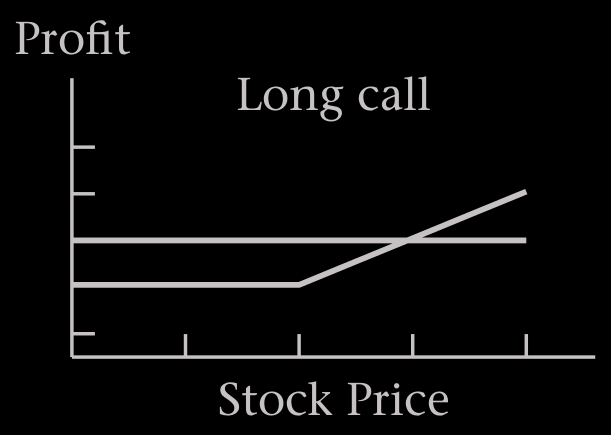
\includegraphics[scale=0.15]{figs/Long-call.png}
		\end{minipage}
		 $ \quad + \quad $
		\begin{minipage}{0.3\textwidth}
			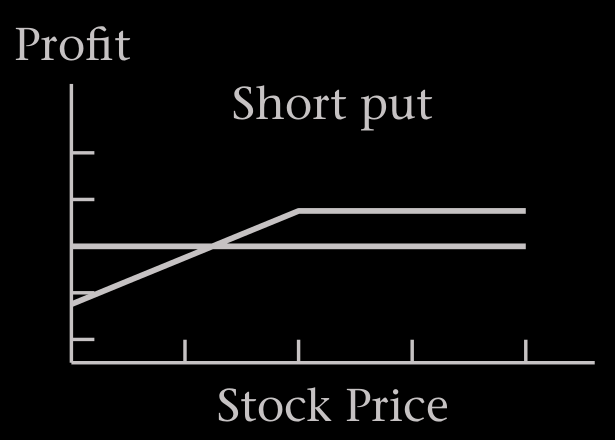
\includegraphics[scale=0.15]{figs/Short-put.png}
		\end{minipage}
	\end{center}
\end{myexample}
\end{frame}
%-------------- end slide -------------------------------%}}}
%-------------- start slide -------------------------------%{{{ 1
\begin{frame}[fragile,t]
	\begin{mysol}
		\begin{center}
			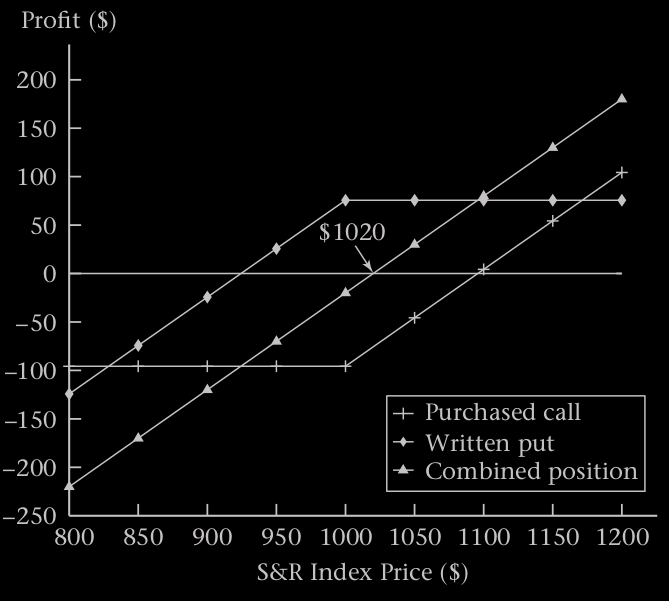
\includegraphics[scale=0.25]{figs/Figure-3-6.png}
		\end{center}
		\myEnd
	\end{mysol}
\end{frame}
%-------------- end slide -------------------------------%}}}
%-------------- start slide -------------------------------%{{{ 1
\begin{frame}[fragile,t]
	\begin{center}

		\textcolor{magenta}{A synthetic long forward contract}\\
		\bigskip

		We pay the net option premium\\[1em]
		We pay the strike price

		\bigskip
		\mySeparateLine
		\bigskip

		\textcolor{cyan}{The actual forward} \\
		\bigskip
		We pay zero premium \\[1em]
		We pay the forward price

\end{center}
\end{frame}
%-------------- end slide -------------------------------%}}}
%-------------- start slide -------------------------------%{{{ 1
\begin{frame}[fragile,t]
\begin{center}
	\textcolor{magenta}{\bf Basic Assumption}\\[1em]
	\bigskip

	The net cost of buying the index using options \\
	\bigskip

	must equal \\
	\bigskip

	the net cost of buying the index using a forward contract.

	\bigskip
	\bigskip
	\bigskip

	\pause
	\textcolor{cyan}{\bf \large NO ARBITRAGE!}

\end{center}
\end{frame}
%-------------- end slide -------------------------------%}}}
%-------------- start slide -------------------------------%{{{ 1
\begin{frame}[fragile]
\begin{center}
	\textcolor{magenta}{\bf The Put-Call parity equation}

	\begin{align*}
		\text{Call}(K,T) - \text{Put}(K,T) = \text{PV}\left(F_{0,T}-K\right)
	\end{align*}
	\pause
	\begin{itemize}
		\item $K$: strike price
		\item $T$: expiration date
		\item $\text{Call}(\cdot,\circ)$: the premium for call.
		\item $\text{Put}(\cdot,\circ)$: the premium for put.
		\item $F_{0,T}$: the forward price at time $T$ if one enters at time $0$ into a long forward position.
		\item $\text{PV}(\cdot)$: the present value function.
	\end{itemize}
\end{center}
\end{frame}
%-------------- end slide -------------------------------%}}}
%-------------- start slide -------------------------------%{{{ 1
\begin{frame}[fragile,t]
\begin{myexample}
	Check	Example \myref{E:3-1-0} to see if the put-call parity equation is satisfied.
\end{myexample}
\bigskip
\pause
\begin{mysol}
	We need to check:
	\begin{align*}
		\$93.809 - \$74.201 \stackrel{?}{=} \text{PV}(\$1,000 \times 1.02- \$1,000)
	\end{align*}
	\pause
	Clearly, $\text{LHS}=\$19.61$. \pause On the other hand, the RHS is equal to
	\begin{align*}
		\text{PV}(\$1,000 \times 1.02- \$1,000) & = \text{PV}\left(1,000 \times (1.02-1)\right) \\
                                            & = \text{PV}\left(1,000 \times 0.02\right)     \\
                                            & = \frac{1,000 \times 0.02}{1.02}              \\
																						& = \$19.61.
	\end{align*}
	\pause
	Hence, the put-call parity equation is satisfied.\myEnd
\end{mysol}
\end{frame}
%-------------- end slide -------------------------------%}}}
%-------------- start slide -------------------------------%{{{ 1
\begin{frame}[fragile,t]
	\begin{gather*}
		\textcolor{gray}{\text{Call}(K,T) - \text{Put}(K,T) = \text{PV}\left(F_{0,T}-K\right)} \\[1em]
		\textcolor{gray}{\Updownarrow}\\[1em]
		\text{PV}\left(F_{0,T}\right) +	\text{Put}(K,T) = \text{Call}(K,T) + \text{PV}\left(K\right)
	\end{gather*}

	\bigskip
	\mySeparateLine
	\bigskip

	\begin{center}
		Buying the index and buying the put \\
		\bigskip
		generate the same payoff as\\
		\bigskip
		buying the call and buying a zero-coupon bond (i.e. lending) $\text{PV}(K)$
	\end{center}
\end{frame}
%-------------- end slide -------------------------------%}}}
%-------------- start slide -------------------------------%{{{ 1
\begin{frame}[fragile,t]
	\begin{gather*}
		\textcolor{gray}{\text{Call}(K,T) - \text{Put}(K,T) = \text{PV}\left(F_{0,T}-K\right)} \\[1em]
		\textcolor{gray}{\Updownarrow}\\[1em]
		\text{PV}\left(F_{0,T}\right) -	\text{Call}(K,T) = \text{PV}\left(K\right)-\text{Put}(K,T)
	\end{gather*}

	\bigskip
	\mySeparateLine
	\bigskip

	\begin{center}
		Writing a covered call\\
		\bigskip
		has the same profit as\\
		\bigskip
		lending $\text{PV}(K)$ and selling a put
	\end{center}
\end{frame}
%-------------- end slide -------------------------------%}}}
%-------------- start slide -------------------------------%{{{ 1
\begin{frame}[fragile,t]
	\begin{gather*}
		\textcolor{green}{\text{Call}(K,T)} - \textcolor{cyan}{\text{Put}(K,T)} =
		\textcolor{magenta}{\text{PV}\left(F_{0,T}\right)}-\textcolor{yellow}{\text{PV}\left(K\right)}
	\end{gather*}

	\bigskip
	\mySeparateLine
	\bigskip
	\begin{center}
		Revisit four positions in Section 3.1\\

		\bigskip

\renewcommand{\arraystretch}{1.2}
		\begin{tabular}{|c|c|c|}
			\hline
			 Position                         & Meaning                                                              & equivalent to                                                        \\ \hline
			 Inuring a long position (floors) & \only<2->{\textcolor{magenta}{Index} $+$ \textcolor{cyan}{Put}}      & \only<3->{\textcolor{yellow}{Bound} $+$ \textcolor{green}{Call}}     \\
			 Inuring a short position (caps)  & \only<4->{$-$\textcolor{magenta}{Index} $+$ \textcolor{green}{Call}} & \only<5->{$-$\textcolor{yellow}{Bound} $+$ \textcolor{cyan}{Put}}    \\
			 Covered call writing             & \only<6->{\textcolor{magenta}{Index} $-$ \textcolor{green}{Call}}    & \only<7->{\textcolor{yellow}{Bound} $-$ \textcolor{cyan}{Put}}       \\
			 Covered put writing              & \only<8->{$-$\textcolor{magenta}{Index} $-$ \textcolor{cyan}{Put}}   & \only<9->{$-$ \textcolor{yellow}{Bound} $-$ \textcolor{green}{Call}} \\ \hline
			 \end{tabular}

	\end{center}
\end{frame}
%-------------- end slide -------------------------------%}}}
